\chapter{Manual Usuario}

\section{Página de Inicio}

Es la primera vista, ver figura \ref{fig:home_view}, que se despliega cuando accedemos a la aplicación, se puede ver una descripción del sistema implementado, se pueden apreciar los siguientes elementos:

\begin{enumerate}
  \item Icono del Menú.
  \item Icono del Login o Registro del Usuario.
  \item Botones de Registro de Usuario y Login respectivamente.
\end{enumerate}

\begin{figure}[H]
      \begin{center}
        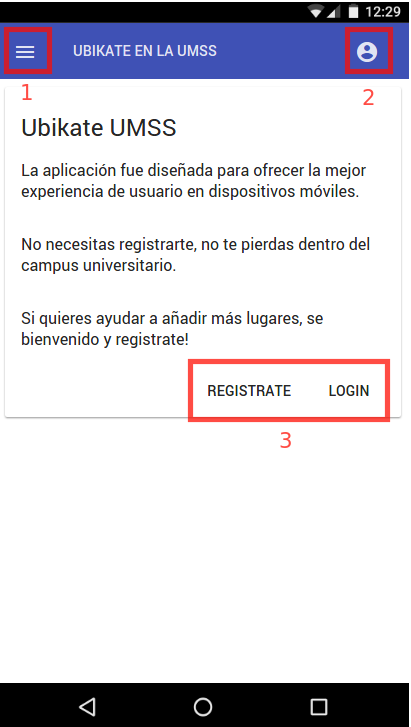
\includegraphics[width=0.3\textwidth]{manual_usuario/home}

        \caption{Página de Inicio.}
        \label{fig:home_view}
        \caption*{Fuente: Elaboración propia.}
      \end{center}
\end{figure}

\section{Menu de la Aplicación}

Está ubicado en el sección izquierda de la pantalla, se accede a ella haciendo un tap sobre el \emph{icono del Menú}, ver la figura \ref{fig:menu_view}. Una vez que se selecciona cualquier opción del menú, este se oculta. De esta forma se aprovecha el espacio reducido que dispone un dispositivo móvil.


\begin{figure}[H]
      \begin{center}
        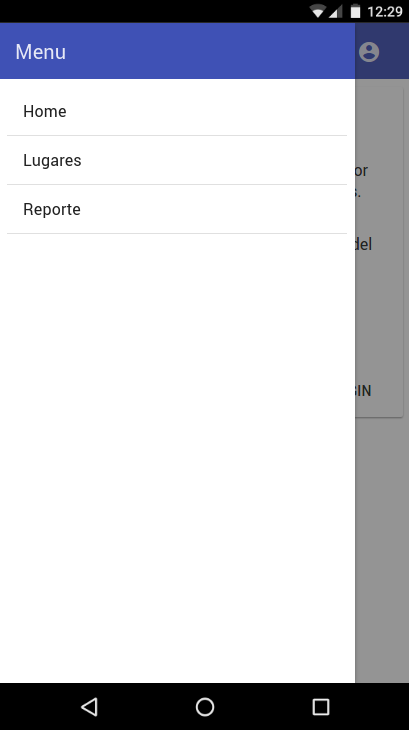
\includegraphics[width=0.3\textwidth]{manual_usuario/menu}

        \caption{Menú de la aplicación.}
        \label{fig:menu_view}
        \caption*{Fuente: Elaboración propia.}
      \end{center}
\end{figure}


\section{Lista de Lugares}

Se accede a la \emph{lista de lugares}, ver figura \ref{fig:vista_lugares}, seleccionando la opción \emph{Lugares} del Menú.

En la \emph{lista de lugares} se puede ver los siguiente elementos:

\begin{enumerate}
  \item Cajón de Búsqueda.
  \item Lista de Lugares.
  \item Botón de Registro de un Lugar (ver figura \ref{fig:vista_search}).
\end{enumerate}

\begin{figure}[H]
      \begin{center}
        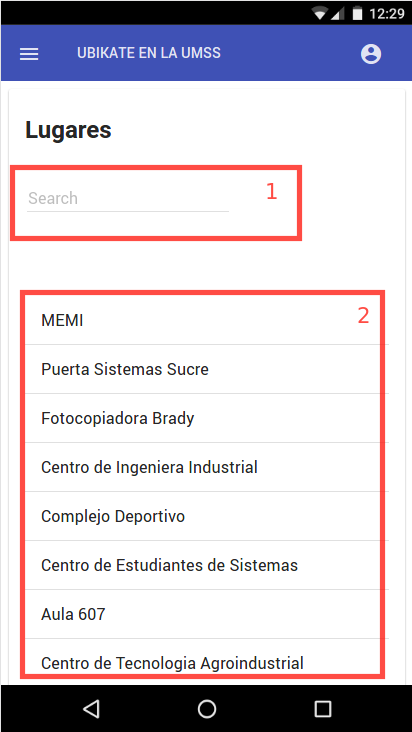
\includegraphics[width=0.3\textwidth]{manual_usuario/lugares}

        \caption{Lista de lugares.}
        \label{fig:vista_lugares}
        \caption*{Fuente: Elaboración propia.}
      \end{center}
\end{figure}

\begin{itemize}
  \item \textbf{Cajón de Búsqueda:} La lista de lugares es filtrada de acuerdo al nombre de un lugar o parte del nombre, que es ingresada en el \emph{cajón de búsqueda}. Como se puede apreciar en la figura \ref{fig:vista_search}.

  \begin{figure}[H]
        \begin{center}
          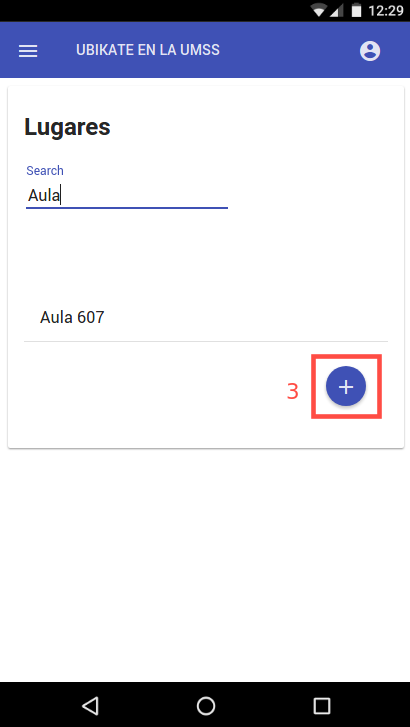
\includegraphics[width=0.25\textwidth]{manual_usuario/search}

          \caption{Cajón de Búsqueda.}
          \label{fig:vista_search}
          \caption*{Fuente: Elaboración propia.}
        \end{center}
  \end{figure}

  \item \textbf{Lista de Lugares:} Es la lista de lugares propiamente dicha, contiene todos los lugares registrados en la aplicación o la lista filtrada mediante el \emph{cajón de búsqueda}.

\item \textbf{Botón de Registro de un Lugar:} Ubicada al final de la \emph{lista de lugares}.

\end{itemize}

\section{Formulario de registro de un Lugar}

El \emph{formulario de registro de un lugar} contiene la siguiente información:
\begin{enumerate}
  \item El \emph{Nombre} del lugar, esta información es requerida.
  \item La \emph{Descripción} del lugar, en caso de que tuviera una, no es requerida.
  \item El \emph{Teléfono} del lugar, en caso de que tuviera una.
  \item El \emph{Nivel} o \emph{Piso} de donde se encuentra lugar, si no es especifica un piso, el sistema deduce que el lugar está en el \emph{nivel 0} o \emph{Planta Baja}.
\end{enumerate}

\begin{figure}[H]
      \begin{center}
        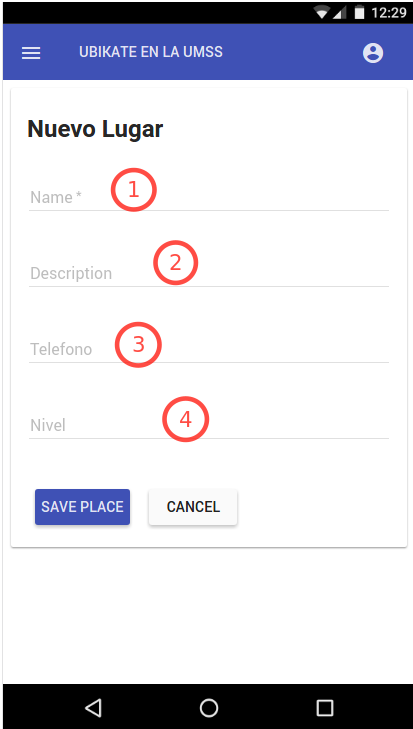
\includegraphics[width=0.3\textwidth]{manual_usuario/registro_place}

        \caption{Formulario de Registro de un Lugar.}
        \label{fig:vista_registro_place}
        \caption*{Fuente: Elaboración propia.}
      \end{center}
\end{figure}

\section{Información del Lugar}

La \emph{información de un lugar}, ver la figura \ref{fig:vista_información_lugar}, contiene los siguientes datos:
\begin{enumerate}
  \item La \emph{Foto} o imagen del lugar.
  \item La \emph{Información} del lugar, todos los datos ingresados en el \emph{formulario de registro}.
  \item El \emph{Botón para agregar imagenes} del lugar, las imágenes agregadas serán desplegadas en la parte superior de la \emph{información del lugar}.
  \item El \emph{Botón para encontrar la Ruta óptima al lugar}, al seleccionar esta opción se despliega el mapa del campus Universitario. Ver la figura \ref{fig:vista_ruta}.
  \item El \emph{Botón para Editar la Información del lugar}, al seleccionar esta opción se despliega el \emph{Formulario de edición de un Lugar}.
\end{enumerate}


\begin{figure}[H]
      \begin{center}
        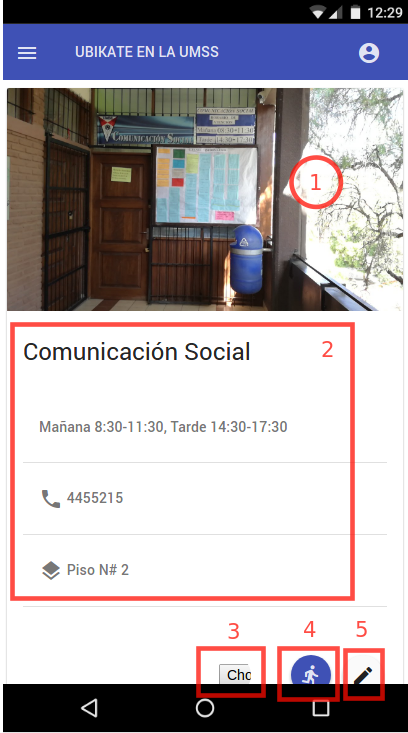
\includegraphics[width=0.25\textwidth]{manual_usuario/informacion_lugar}

        \caption{Información de un Lugar.}
        \label{fig:vista_información_lugar}
        \caption*{Fuente: Elaboración propia.}
      \end{center}
\end{figure}


\begin{figure}[H]
      \begin{center}
        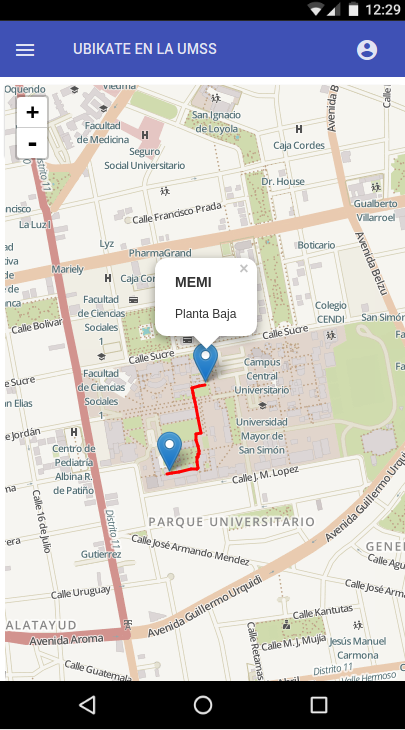
\includegraphics[width=0.25\textwidth]{manual_usuario/ruta}

        \caption{Vista del camino o ruta óptima al lugar.}
        \label{fig:vista_ruta}
        \caption*{Fuente: Elaboración propia.}
      \end{center}
\end{figure}


% \begin{figure}[H]
%   \centering
%   \begin{minipage}[b]{0.3\textwidth}
%     \includegraphics[width=\textwidth]{manual_usuario/información_lugar}
%     \caption{Información de un Lugar.}
%     \label{fig:vista_información_lugar}
%     % \caption*{Fuente: Elaboración propia.}
%   \end{minipage}
%   % \hfill
%   % \hspace*{3cm}
%   \blank{3cm}
%
%   \begin{minipage}[b]{0.3\textwidth}
%     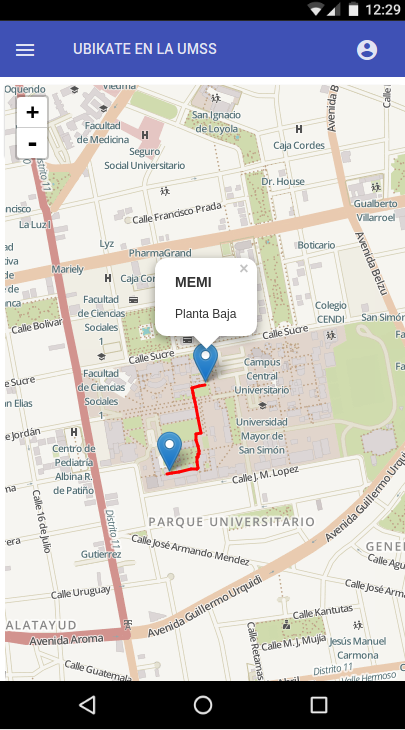
\includegraphics[width=\textwidth]{manual_usuario/ruta}
%     \caption{Vista del camino o ruta óptima al lugar.}
%     \label{fig:vista_ruta}
%     % \caption*{Fuente: Elaboración propia.}
%   \end{minipage}
%   \caption*{Fuente: Elaboración propia.}
%
% \end{figure}


\section{Formulario de edición de un Lugar}

El \emph{formulario de edición de un lugar} contiene la misma información que el \emph{formulario de registro de un lugar}, pero en el formulario de edición está desplegada la información del lugar para ser edita, ver la figura \ref{fig:vista_edicion_lugar}.

\begin{figure}[H]
      \begin{center}
        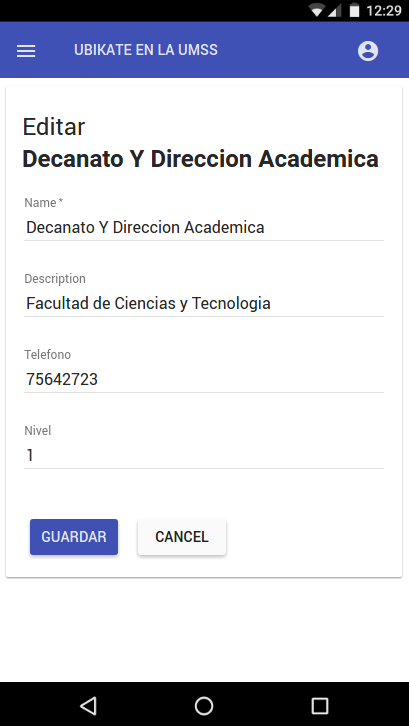
\includegraphics[width=0.25\textwidth]{manual_usuario/edicion}

        \caption{Formulario de edición de un lugar.}
        \label{fig:vista_edicion_lugar}
        \caption*{Fuente: Elaboración propia.}
      \end{center}
\end{figure}



\section{Formulario de registro de un Usuario}

Dentro del \emph{formulario de registro de un usuario} todos los campos son necesario, en caso de no ingresar un dato, la aplicación muestra un mensaje indicando que el campo es requerido. Como se puede ver en la figura \ref{fig:vista_registro_user}, dentro de este formulario se pueden ver los siguientes campos:
\begin{enumerate}
  \item El \emph{Nombre} del usuario.
  \item El \emph{Email} del usuario.
  \item La \emph{Razón} o el \emph{Porque} del registro.
\end{enumerate}

\begin{figure}[H]
      \begin{center}
        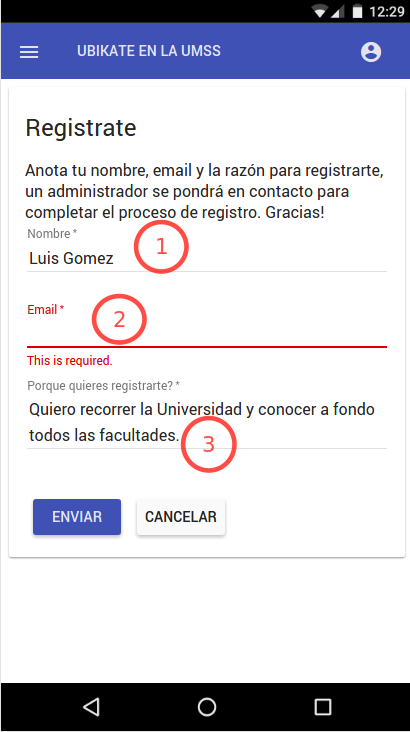
\includegraphics[width=0.25\textwidth]{manual_usuario/registro_usuario}

        \caption{Formulario de registro de un Usuario.}
        \label{fig:vista_registro_user}
        \caption*{Fuente: Elaboración propia.}
      \end{center}
\end{figure}


\section{Formulario de ingreso al sistema}

El \emph{formulario de ingreso al sistema} o \emph{Login}, ver figura \ref{fig:vista_login}, nos permite acceder al sistema con permisos de \emph{Administrador} o de \emph{Usuario Registrado}.

\begin{figure}[H]
      \begin{center}
        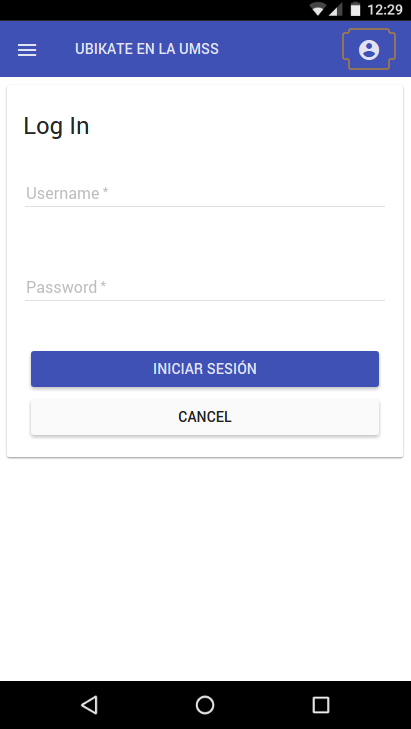
\includegraphics[width=0.25\textwidth]{manual_usuario/login}

        \caption{Formulario de ingreso al sistema.}
        \label{fig:vista_login}
        \caption*{Fuente: Elaboración propia.}
      \end{center}
\end{figure}


\section{Reporte}

El \emph{Reporte} mostrado en la figura \ref{fig:vista_reporte}, muestra los lugares más visitados por los usuarios de la aplicación, para acceder a él es necesario seleccionar la opción \emph{Reporte} del Menú.

\begin{figure}[H]
      \begin{center}
        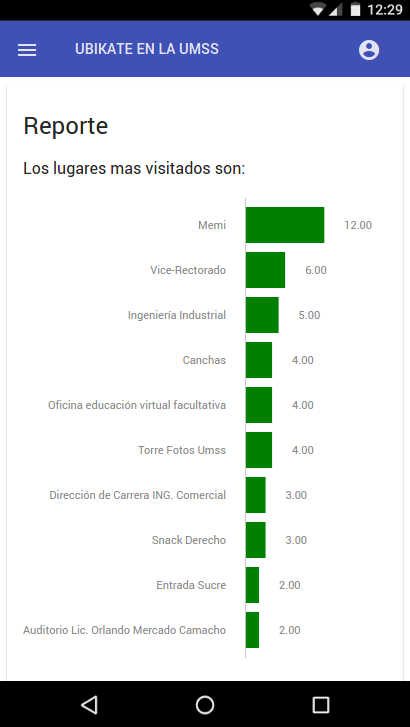
\includegraphics[width=0.25\textwidth]{manual_usuario/reporte}

        \caption{Lugares más visitados.}
        \label{fig:vista_reporte}
        \caption*{Fuente: Elaboración propia.}
      \end{center}
\end{figure}
